% Created 2015-06-16 Ter 00:27
\documentclass[11pt]{article}
\usepackage[utf8]{inputenc}
\usepackage[T1]{fontenc}
\usepackage{fixltx2e}
\usepackage{graphicx}
\usepackage{longtable}
\usepackage{float}
\usepackage{wrapfig}
\usepackage{rotating}
\usepackage[normalem]{ulem}
\usepackage{amsmath}
\usepackage{textcomp}
\usepackage{marvosym}
\usepackage{wasysym}
\usepackage{amssymb}
\usepackage{hyperref}
\tolerance=1000
\usepackage{minted}
\author{Alice}
\date{\today}
\title{arvore\_de\_maxima\_parcimonia}
\hypersetup{
  pdfkeywords={},
  pdfsubject={},
  pdfcreator={Emacs 24.4.1 (Org mode 8.2.10)}}
\begin{document}

\maketitle
\tableofcontents

\section{Enunciado}
\label{sec-1}

\textit{Reconstruindo árvores filogenéticas pelo método da máxima parcimônia}

Uma árvore filogenética é uma árvore em que as folhas são espécies
diferentes, cuja raiz é o ancestral comum de tais espécies e cujos
galhos representam eventos de especiação.

Queremos achar:

\begin{itemize}
\item Uma árvore (binária) evolucionária com as espécies dadas
\item Para cada nó interno uma string de comprimento $k$ com a
sequência genética daquele ancestral.
\end{itemize}


Dada uma árvore acompanhada de uma string $s(u) \in \{A, C, G, T\}^k$ para
cada nó $u \in V(T)$, podemos atribuir uma nota usando o método da
máxima parcimônia, que diz que menos mutações são mais prováveis:
\[ \mathrm{nota}(T) = \sum_{(u,v) \in E(T)} (\text{número de posições em que }s(u)\text{ e }s(v)\text{ diferem}). \]

Achar a árvore com nota mais baixa é um problema difícil. Aqui vamos
considerar um problema menor: Dada a estrutura da árvore, achar as
sequências genéticas $s(u)$ para os nós internos que dêem a nota mais
baixa.

Um exemplo com $k = 4$ e $n = 5$:

\href{http:github.com/adusca/FGV-EDA/6_30/tree.png}{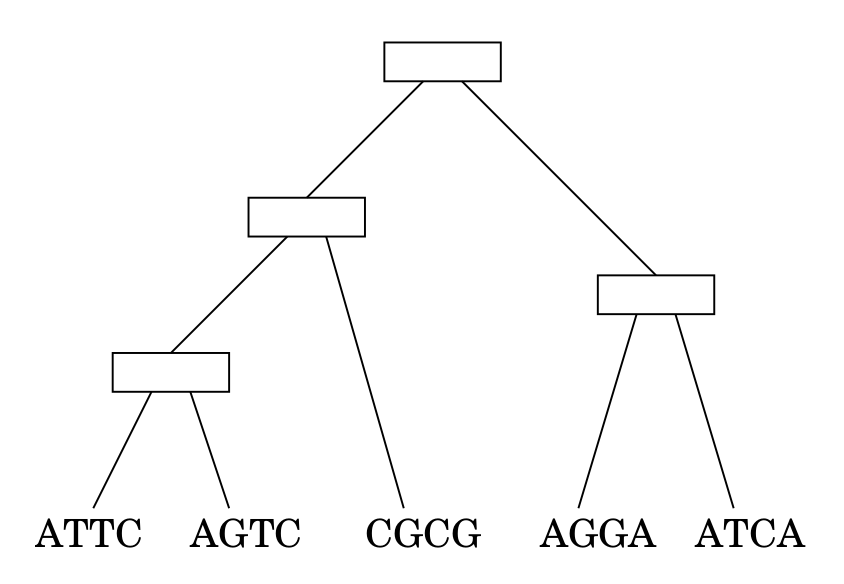
\includegraphics[width=.9\linewidth]{tree.png}}

\begin{enumerate}
\item Ache uma reconstrução para o exemplo seguindo o método da
máxima parcimônia.
\item Dê um algoritmo eficiente para essa tarefa.
\end{enumerate}


\section{Dados reais}
\label{sec-2}

Usamos \url{http://www.ncbi.nlm.nih.gov/Taxonomy/CommonTree/wwwcmt.cgi} para gerar o banco de dados.

Rosalind MULT, GLOB, EDTA, PERM, EDIT, LCSQ,
CSTR, CTBL, NWCK, SSET, MRNA, KMP, PROB
SSEQ, SPLC, LCSM
% Emacs 24.4.1 (Org mode 8.2.10)
\end{document}
